

\begin{mydef}
	Un angle est défini par \hspace*{8cm}. 
	
	Les demis droites sont les \hspace{3cm} de l'angle et leur origine est son \hspace{4cm}.
\end{mydef}

\begin{myex}
	\begin{multicols}{2}
		Cet angle est défini par les demi-droites $[BA)$ et $[BC)$. \hspace*{4cm} sont ses cotés et \hspace{1cm} est son sommet.
		On le note $\widehat{ABC}$ (le sommet de l'angle est toujours au milieu).
		
		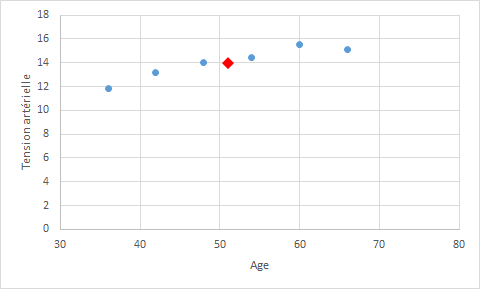
\includegraphics[scale=0.2]{ex1}
	\end{multicols}
\end{myex}